\section{The Lot of Fortune and its Relationship to the Topic “Length of Life,” with Examples. Included are the Minimum Periods of the Stars (14K,11P)}

I have found this system for $<$finding$>$ the length of life to have been elaborated in a very complicated manner by the ancients. After investigation, I have modified their doctrines in view of my experience, and I think $<$my explanations$>$ will please most $<$of my readers$>$. 

In his thirteenth book, after his preface and his descriptions of the signs, the King introduces the Lot of Fortune $<$and its derivation$>$ from the \Sun, the \Moon, and the Ascendant. He considers it the be the greatest, and he mentions it throughout his work, calling it the “Ruling Place.” He makes a great mystery of its “forward and reverse”: 
\begin{quote}
The Sun, starting in the dawn and declining to his western arc, opens $<$to us$>$ the vault of the cosmos, as can be seen. When night arrives, the Moon will not always become the Lightbringer, but sometimes \textbf{/155K/} it appears in the West, setting, sometimes it stays in the heavens for quite a while, at other times it travels the entire night. As a result, the whole circle $<$of the zodiac$>$ has rightly /147P/ been entrusted to the Sun’s care.
\end{quote}

There are a variety of opinions about this notion. To me it seems best to locate the Lot by determining the distance from the \Sun\xspace to the \Moon, then counting that distance from the Ascendant—for day births. 

For night births $<$1$>$ if the Moon is above the earth, i.e. until the time it sets, determine the distance from it to the \Sun, then count that distance from the Ascendant. $<$2$>$ After the moon has set, determine the distance from the \Sun\xspace to it. 

As for the king’s final statement: “The whole circle $<$of the
zodiac$>$ has been entrusted to the Sun’s care,” this seems correct. 

It will be necessary to examine the place where the Lot is located, and to consider that place to be the ruler. Then determine in which sign the ruler of the sign $<$of the Lot$>$ happens to be located. Third, determine that sign’s houseruler. From these three places and from their houserulers the native’s length of life will be found by using the three factors.

Each star controls its own period: 
\begin{center}	
\begin{tabular}{cS}
\toprule
\textbf{Planet} & \textbf{Years} \\
\midrule
\Saturn & 30 \\
\Jupiter & 12 \\
\Mars & 15 \\
\Sun & 19 \\
\Venus & 8 \\
\Mercury & 20 \\
\Moon & 25 \\
\bottomrule
\end{tabular}	
\end{center}
	
Each $<$sign$>$ also controls its own rising times according to the $<$nativity’s$>$ klima. Accordingly it will be necessary to determine for the $<$correct$>$ klima whether the Lot is at an angle and operative, or whether it just precedes or follows an angle. 

Also determine the houserulers of the signs. The Old Astrologer reminds us of this when he says: 
\begin{quote}
Each star, when at an angle, allows the full amount of its times. When not at an angle, it grants its allotment after some deduction from its own numbers.
\end{quote}

These stars allot the full term of their periods and their rising times when they are favorably situated. The fellow members of their sects, when in conjunction, in aspect, or in their own signs, add to the allotment, unless both sects in fact join in the allotment. Thus the $<$Old Astrologer$>$.

First it is necessary to calculate the numbers: hours, days, months, then years. Then use the three factors, minimum, mean, maximum, adding the first to the second, or the second to the third. 

It often happens that one place allots the days, another the months, another the years, all according to the differences among the operative signs and the houserulers, or of the baneful influences and setbacks. 

After allotting the years, they also allot \textbf{/156K/} the same number of months to their chronocratorships.

In the distribution $<$of years$>$ Daimon and the Ascending Place will have the same effects as the Lots whenever the places of the Lots or their rulers are unfavorably situated, particularly when the Lot of Fortune cedes the distribution to Daimon. (Stars can indeed yield to each other; we will show how in a future chapter on the allotment procedure.)
\newpage
\textbf{/148P/} Examples: \Sun, \Venus\xspace in \Cancer, \Moon, Ascendant in \Pisces, \Saturn\xspace in \Sagittarius, \Jupiter in \Capricorn, \Mars\xspace in \Scorpio, \Mercury\xspace in \Leo, the Lot of Fortune in \Cancer which is in Good Daimon
$<$=the V Place of Good Fortune$>$\footnote{\textit{Greek Horoscopes} chart L75 used in section III.6}.

\clearpage
\begin{wrapfigure}[15]{R}{7cm}
\centering
\vspace{-20pt}
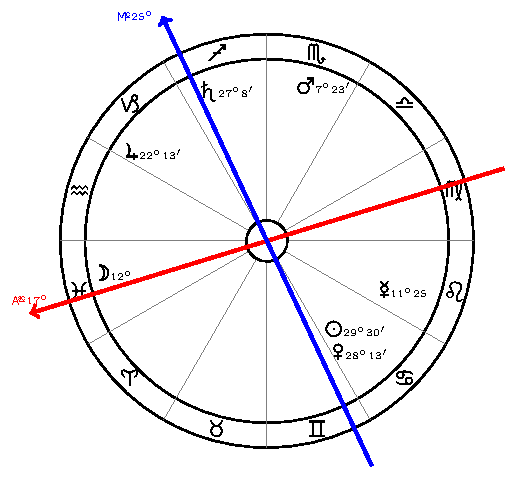
\includegraphics[width=0.68\textwidth]{charts/3_06_1}
\caption{Chart 42a [III.14.1, GH L75]}
\label{fig:chart42a}
\end{wrapfigure}  

The ruler of the Lot $<$moon$>$ was found at an angle. I set down the minimum period for the \Moon, 25 years, plus the rising time of \Cancer\xspace in the second klima, 32 years, plus the period of the houseruler of the \Moon, \Jupiter, 12 years. The total is the same $<$as in Book III.6K$>$, 69
years. The native died at that age.

\newpage
Another example: \Sun\xspace in \Aquarius, \Moon, Ascendant in \Virgo, also \Mars; \Saturn, \Jupiter, \Mercury\xspace in \Capricorn, \Venus\xspace in \Pisces, the Lot of Fortune in \Aquarius\xspace just preceding an angle $<$Descendant$>$
\footnote{\textit{Greek Horoscopes} dates the chart (L135) to approximately January 20, 135 AD (p.126)}.

\clearpage
\begin{wrapfigure}[15]{R}{7cm}
\centering
\vspace{-20pt}
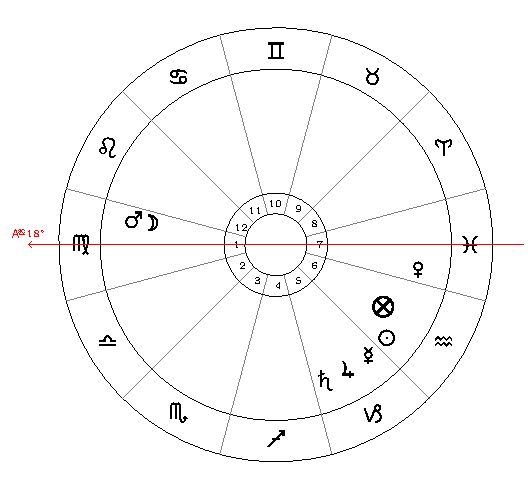
\includegraphics[width=0.68\textwidth]{charts/3_14_2}
\caption{Chart 49 [III.14.2, GH L135]}
\label{fig:chart49}
\end{wrapfigure} 

Its ruler $<$\Saturn$>$ in $<$the V Place of$>$ Good Fortune, not in its own sect $<$diurnal; the nativity is nocturnal$>$
allots its own 30 year period plus the same number of months, since it is in its own sign. \Jupiter, also in this sign, allotted one year $<$12 months$>$. The native died in his 34th year.

For every nativity the rules of procedure laid down previously, the phases, and the degrees, must be observed. $<$I say this$>$ so that we might not seem to be repeating the same reminders with each new topic. For this reason I consider it necessary to cite sample nativities.


\newpage